% `template.tex', a bare-bones example employing the AIAA class.
%
% For a more advanced example that makes use of several third-party
% LaTeX packages, see `advanced_example.tex', but please read the
% Known Problems section of the users manual first.
%
% Typical processing for PostScript (PS) output:
%
%  latex template
%  latex template   (repeat as needed to resolve references)
%
%  xdvi template    (onscreen draft display)
%  dvips template   (postscript)
%  gv template.ps   (onscreen display)
%  lpr template.ps  (hardcopy)
%
% With the above, only Encapsulated PostScript (EPS) images can be used.
%
% Typical processing for Portable Document Format (PDF) output:
%
%  pdflatex template
%  pdflatex template      (repeat as needed to resolve references)
%
%  acroread template.pdf  (onscreen display)
%
% If you have EPS figures, you will need to use the epstopdf script
% to convert them to PDF because PDF is a limmited subset of EPS.
% pdflatex accepts a variety of other image formats such as JPG, TIF,
% PNG, and so forth -- check the documentation for your version.
%
% If you do *not* specify suffixes when using the graphicx package's
% \includegraphics command, latex and pdflatex will automatically select
% the appropriate figure format from those available.  This allows you
% to produce PS and PDF output from the same LaTeX source file.
%
% To generate a large format (e.g., 11"x17") PostScript copy for editing
% purposes, use
%
%  dvips -x 1467 -O -0.65in,0.85in -t tabloid template
%
% For further details and support, read the Users Manual, aiaa.pdf.


% Try to reduce the number of latex support calls from people who
% don't read the included documentation.
%
\typeout{}\typeout{If latex fails to find aiaa-tc, read the README file!}
%


\documentclass[]{aiaa-tc}% insert '[draft]' option to show overfull boxes

\usepackage{lettrine}%  dropped capital letter at beginning of paragraph
\usepackage{subfigure}% subcaptions for subfigures
\usepackage{subfigmat}% matrices of similar subfigures, aka small mulitples
\usepackage{placeins}%  figure section constraint
\usepackage{mathtools}% not sure why this is here...probs for math stuff
\usepackage{graphicx}
\graphicspath{./}
\usepackage{listings}

 \title{Final Project: \\ Poisson's Equation}

 \author{
  Ryan J. Krattiger%
    \thanks{Undergraduate Senior, Department of Mechanical and Aerospace Engineering.} \\
  {\normalsize\itshape
  Missouri University of Science and Technology, Rolla, MO, 65401, USA} \\
  Russley F. Shaw%
    \thanks{Undergraduate Senior, Department of Computer Science.} \\
  {\normalsize\itshape
  Missouri University of Science and Technology, Rolla, MO, 65401, USA}
 }

 % Data used by 'handcarry' option if invoked
 \AIAApapernumber{YEAR-NUMBER}
 \AIAAconference{Conference Name, Date, and Location}
 \AIAAcopyright{\AIAAcopyrightD{YEAR}}

 % Define commands to assure consistent treatment throughout document
 \newcommand{\eqnref}[1]{(\ref{#1})}
 \newcommand{\class}[1]{\texttt{#1}}
 \newcommand{\package}[1]{\texttt{#1}}
 \newcommand{\file}[1]{\texttt{#1}}
 \newcommand{\BibTeX}{\textsc{Bib}\TeX}

\begin{document}

\maketitle

\begin{abstract}

\end{abstract}

\newpage

\tableofcontents

\lstlistoflistings

\newpage

\section*{Nomenclature}

\begin{tabbing}
  XXX \= \kill% this line sets tab stop
  $f$ \> Function \\
  $\bar x$ \> Variable value vector \\
  h \> Step size \\
  x \> x-position \\
  $\bar r$ \> residual vector \\
  \textit{Subscript} \\
  $i$ \> Row index \\
  $j$ \> Column index \\
 \end{tabbing}

% ---------------------------------------------------------------------------- %
%                                     MODEL                                    %
% ---------------------------------------------------------------------------- %
\FloatBarrier\section{Models}

% ----------------------- %
% -- Poisson's Equation --%
% ----------------------- %
\FloatBarrier\subsection{Poisson's Equation}

The poisson eqaution is used in many diciplines as it is a common mathematical
model found in physical systems. Because of the relative complexity of these
physical systems, a simplified and solvable example was used to demonstrate 
two different linear system solvers. The methods presented here are 
Steepest Descent Optimization and Gauss-Seidel Iterations, or as applied to PDE
solvers the Liebmann Method.

The first thing to consider is the general form of Poisson's equation as seen in
Eq~\ref{e:p_diff}. It is clear that this is a second order, linear, partial differential
equation in two dimensions, x and y. The forcing function, f(x,y), can be anything
depending on the problem and is one of five drivers for the solution, including the
four boundary conditions.

\begin{equation}
  \label{e:p_diff}
  \frac{\partial ^2 u}{\partial x^2} + \frac{\partial ^2 u}{\partial y^2} = f(x,y)
\end{equation}

Being a second order PDE, it is required to have two boundary conditions for each
independent variable. In this case that would be x and y, resulting in the required
four boundary conditions.

For the current problem, the forcing function can be seen in Eq~\ref{e:p_f}
and the boundary conditions are writen in Eq~\ref{e:p_bcx} and Eq~\ref{e:p_bcy}.

\begin{equation}
  \label{e:p_f}
  f(x,y) = -2(x^2 + y^2)\quad \textrm{for} \quad (0 \leq x \leq 1, 0 \leq y \leq 1)
\end{equation}

\begin{equation}
  \label{e:p_bcx}
  u(x,0) = 1 - x^2 \quad \textrm{,} \quad u(x,1) = 2(1 - x^2) \quad \textrm{for} \quad 0 \leq x \leq 1
\end{equation}

\begin{equation}
  \label{e:p_bcy}
  u(0,y) = 1 + y^2 \quad \textrm{,} \quad u(1,y) = 0 \quad \textrm{for} \quad 0 \leq y \leq 1
\end{equation}

It can be shown that the exact solution for these constraints is as seen in Eq~\ref{e:p_exact}.

\begin{equation}
  \label{e:p_exact}
  u(x,y) = (1 - x^2)(1 + y^2)
\end{equation}

The set up of the problem is independent of any set of inputs.

This first step is to descretize the original PDE as seen in Eq~\ref{e:p_diff} into
the form seen in Eq~\ref{e:p_num}. It can be seen that the second order, central
difference scheme was used.
\\\\
Let $u(x_i,y_j) = u_{i,j}$, where $i \in [0,N]$, $j \in [0,M]$, and $h = \frac{x_N - x_0}{N}$ and $k = \frac{y_M - y_0}{M}$

\begin{equation}
  \label{e:p_num}
  \frac{u_{i-1,j} - 2u_{i,j} + u_{i+1,j}}{h^2} + \frac{u_{i,j-1} - 2u_{i,j} + u_{i,j+1}}{k^2} = f(x_i,y_j)
\end{equation}

Further simplifying this equation and letting $\frac{h^2}{k^2} = \lambda$ gives a
general simplified form for the numerical scheme (Eq~\ref{e:p_num_simp}). For this
solver, it will be assumed that h and k are the same, or the grid is square and
equally spaced. This is a constraint of the current implementation.

\begin{equation}
  \label{e:p_num_simp}
  - 2(\lambda + 1)u_{i,j} + \lambda u_{i-1,j} + \lambda u_{i+1,j}  + u_{i,j-1} + u_{i,j+1} = f(x_i,y_j)
\end{equation}

After some carefull consideration it can be shown that the above eqation can be
applied to the grid structure in figure~\ref{f:cdiff_grid}. It can also be seen
that at the boundaries, where the values are known from boundary conditions, can
be looked at as constants.

\begin{figure}
  \centering
  \label{f:cdiff_grid}
  \caption{Grid with points used in central difference discretized Poisson}
  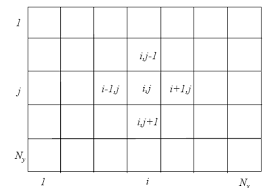
\includegraphics[width=0.5\textwidth]{cdiff_grid.png}
\end{figure}

In order to put the now discretized equation into a solvable form it is translated
to a system of linear equations and can be written in the form of $A \bar x = \bar b$.
\\\\
A is a MxM tridiagonal block matrix with blocks of size NxN. In total it is a 
(NxM)x(NxM) matrix.
$$
\begin{bmatrix}
  T      & I     &     0   & \dots & 0 \\
  I     & T      & I     &  & \vdots \\
  0 &  & \ddots &  & 0 \\
  \vdots &   & I     & T & I \\
  0      & \dots  &  0     & I & T
\end{bmatrix}
$$
\\\\
and T is a NxN tridiagonal matrix
$$
\begin{bmatrix}
  -2(\lambda + 1)      & \lambda     &     0   & \dots & 0 \\
  \lambda     & -2(\lambda + 1)      & \lambda     &  & \vdots \\
  0 &  & \ddots &  & 0 \\
  \vdots &   & \lambda     & -2(\lambda + 1) & \lambda \\
  0      & \dots  &  0     & \lambda & -2(\lambda + 1)
\end{bmatrix}
$$
\\\\
and I is an NxN identity matrix.

In total, A is (NxM)x(NxM) which is quite large. To handle this, we developed a 
contiguous banded matrix that supports upper and lower bands as well as the diagonal.
In total, the relative storage is fractional in comparison to a traditional dense
matrix for this problem. The total data storage is now NxNx(Number of bands) in 
a dense matrix.

The $\bar b$ vector is composed of two parts. This first is made up of the boundary
conditions ($\bar c$), and the second is the forcing vector ($\bar d$). The resulting
$\bar b$ is the denoted as $\bar b = \bar c  + \bar d$.
\\\\
$\bar c$ can be defined as

$$
\begin{bmatrix}
  -( u_{1,0} + \lambda u_{0,1}) \\
  -u_{2,0} \\
    \vdots \\
  -( u_{N-1,0} + \lambda u_{N,1}) \\
  \lambda u_{0,2} \\
    0 \\
  \vdots \\
    0 \\
  \lambda u_{N,2} \\
  \vdots \\
  -( u_{1,M} + \lambda u_{0,M-1}) \\
  -u_{2,M-1} \\
    \vdots \\
  -( u_{N-1,M} + \lambda u_{N,M-1}) \\
\end{bmatrix}
$$
\\\\
$\bar d$ can be defined as

$$
\begin{bmatrix}
  f(x_1,y_1) \\
  f(x_1,y_2) \\
  \vdots \\
  f(x_{N-1},y_{M-1})
\end{bmatrix}
$$
\\\\
And finally $\bar x$, the solution vector is the set of unknown nodes on the grid.
The (i,j) coordinate of the grid is translated using a linear relation to give
a vectorized form of the matrix such that

$$
\begin{bmatrix}
  u_{1,1} \\
  u_{1,2} \\
  u_{1,3} \\
  \vdots \\
  u_{N-1,M-1}
\end{bmatrix}
$$

In the final form of $A \bar x = (\bar c + \bar d)$ the Poisson equation is in a
form that is solvable using afore mentioned linear system solving techniques.

\subsubsection{Liebmann Method}
As an iterative solving technique, Liebmann Method, also known as the Gauss-Seidel method,
is best applied to sparse structured matrices rather than dense matrices. The reason
for this is due to the need to perform O(N$^{2}$) operations, or one operation for
each non zero element of the matrix, to compute the values of $\bar x$ in each iteration.
If there are many non-zero values, there are more operations required for each iteration.
Since the matrix proposed above is indeed sparse, this method is more desirable than a
traditional Gauss-Eliminiation technique. Selecting an initial guess, say the $\bar b$
vector from above, it is possible to now begin iterations.

For iteration k+1, the general form for the x$_i$ element is Eq~\ref{e:lieb_it} for $i\in 0...N$
and N is the size of the solution vector.

\begin{equation}
  \label{e:lieb_it}
  x_i^{k+1} = \frac {b_i - \sum_{j=0}^{i-1} x_j^{k+1} a_{i,j} - \sum_{j=i+1}^{N} x_j^k a_{i,j}}{a_{i,i}}
\end{equation}

In implementation the solution vector would be a single variable, so as $x_i$ was
updated, the update would be seen when solving for $x_{i+1}$. With this in mind,
the above Eq~\ref{e:lieb_it} can be changed into a simpler form seen in Eq~\ref{e:lieb_it2},
recalling that the projection of two vectors (or the dot product) is
$\bar a \cdotp \bar b = \sum_{i=0}^{N} a_i b_i$. Also let $\bar a_i$ be the vector
created by the i$^{th}$ row of the matrix A.

\begin{equation}
  \label{e:lieb_it2}
  x_i = \frac {b_i - \bar a_{i} \cdotp \bar x + a_{i,i} x_i}{a_{i,i}}
\end{equation}

By iterating of Eq~\ref{e:lieb_it2} until convergence of the residual vector
$\vert\vert r_k \vert\vert_2 \leq tolerance$.
The reason to rewrite the solver in this way is to give way to allow the underlying
operation of the dot product be optimized for sparse vector types. In this sense, for
each product of the A matrix row and the current solution vector, a minimum number
of operations will be performed. This also allows for the solver to work for multiple
types of matrix problems and still obtain optimal performance without having to
write a special solver for every sparse or dense matirx used. The same idea will
be used again in the the next solver. In the implementation of this method is was named
Gauss-Seidel to reflect the general form of the solver. Here, it was called Leibmann
simply due to its use with PDEs.

\subsubsection{Steepest Descent}
Another iterative solver can be used, however the Steepest Descent method looks
at this problem as an optimization problem rather than a system of linear equations
solving problem.

In general an optimization problem for a function F($\bar x$) is as follows:
\\\\
Determine a search direction $\bar s_k$
\\\\
Solve for the optimal $\alpha_k^{*}$ to find to minimum in the search direction
use the knowns $\bar x_k$ and the search direction $\bar s_k$ and then use 1D minimization
on F($x_{k+!}$($\alpha_k^{*}$)). The below is an example of using the derivative
of F to find the minimum.

$$
   F'(\bar x_{k+1}) = 0 \quad \textrm{where} \quad \bar x_{k+1} = \bar x_{k} + \alpha_k^{*} \bar s_k
$$


Finally update $\bar x$
$$
   \bar x_{k+1} = \bar x_{k} + \alpha_k^{*} \bar s_k
$$

and check if the solution meets convergence criteria using the norm of the
residual vector ($\bar r_k = A \bar x_k - \bar b$).
$$
\vert\vert r_k \vert\vert_2 \leq tolerance
$$

The current problem to be solved is $Ax-b=\bar 0$; however, a linear system is not a form that
is particularly well suited for optimization since the zero vector is not the
minimum. By integrating the system the resulting equation is $\frac{1}{2} x^T A x - x^T b = 0$.
This form of the equation does have a minimum as it is a quadratic system of eqations.
\\\\
For the Steepest Descent method, the search direction is determined by the local
direction of steepest descent, or the negative gradient. The formula for this should look
familiar as Eq~\ref{e:p_sk}, which is the residual vector.

\begin{equation}
  \label{e:p_sk}
  \bar s_k = \bar r_k = \bar b - A \bar x_k
\end{equation}

The $\alpha_k$ can be found from the above method finding the root of the derivative
as

$$
  \alpha_k = \frac{s_k \cdotp s_k}{s_k \cdotp \bar q_k}
$$

where $\bar q_k = A s_k$.
\\\\
With the search direction ($s_k$) and optimal $\alpha_k^*$ it is a simple matter
to update the solution vector. Again, this will iterator until convergence is
found on the residual vector.

There are two additional methods that are linked to Steepest decent. The first is
Conjugant Gradient (CGM) and the second is Preconditioned Conjugant Gradient (PCGM).
These methods both provide much faster convergence on average, but require more computations
per step. More informatoin about these, and a brief study on how they improve the
gradient based methods as applied to the solution of 2D Poisson's equation
can be found in Holmes et. al.\cite{holmes:07bk}. It would be an excelent addition
to this library to add these improved methods.

\FloatBarrier\subsection{Data Structures}
The foundation of all of the container data structures in this library is the 
specialized mathematical vector named Vector. The vector is dynamically allocated 
and resizeable using smart resizing techniques.

\FloatBarrier\subsubsection{Matrices}
The matrix classes begin with an abstract base class called AMatrix. The AMatrix
not only outlines the common functionality between all matrix types, but also defines
base implementations for many of these functions based on the assumption that a derived
matrix class will define the accessor get(row, col) and mutator set(row, col, value).
These implementations are usually not ideal for the specialized derived matrices;
however, they provide us with a correct implementation with the ability to specialize
further later.

The first specialization of the AMatrix is a dense matrix called the DenseMatrix.
The DenseMatrix specializes in densly packed elements in a matrix. Because of the
assumptions that the AMatrix makes about the definitions of the accessors and mutators,
the DenseMatrix's implementation of methods are similar enough to AMatrix's where
we can simply use the majority of the functionality provided by AMatrix.
The DenseMatrix holds the data internally as a one-dimensional Vector which we access
in a row-column fashion. The same holds true for the mutator operations. Because of the denseness of the matrix, we must hold all elements. Therefore, a given DenseMatrix of size MxN will hold MxN elements. The importance  of the DenseMatrix to our library is that other matrix specialzations may use it as their own internal data storage (i.e. BandedMatrix).

The next specialization of the AMatrix is the SymmetricMatrix, which specializes
in operating on densely packed symmetic data. It utilizes a one dimensional Vector to contain all the elements. Because of this, given an MxM SymmetricMatrix, the Vector only holds $\frac{M(M+1)}{2}$ elements. The importance of the SymmetricMatrix - other than providing a container for dense, symmetric data - is that both upper and lower triangular matricies derive from SymmetricMatrix. These Matricies are names UpperTriMatrix and LowerTriMatrix respectivley. The triangular matricies operate the same as the symmetric matrix, but take advantage of virtual inheritence by being able to hide the SymmetricMatrix's accessor and mutator functionality in substitution of its own. Specifically, the UpperTriMatrix is able to restrict modification and evaluate as zero for its lower half and vice versa for the LowerTriMatrix.

For modelling the linear system generated by discretizing Poisson's Equation, an implementation of the banded matrix is needed. Our library's implmentation is named BandedMatrix. This banded matrix is specialized to be contiguous and dense along the bands. The BandedMatrix is formulated by providing it the row and column, as well as a number of upper bands and a number of lower bands. Given X lower bands and Y upper bands, our data structure allocates Nx(X+Y+1) elements for the X \& Y bands and the diagonal. It additionally leverages optimizations for matrix access and multiplication. Included is also a getPtr(row, col), which returns a C++ pointer. This was included for operations that require many accesses to the underlying data. In addition to the BandedMatrix, a specialization is derived from it called the TridiagMatrix, which is simply a contiguous tridiagonal matrix. This specialization only requires modification of the derived type's constructor. 

% ---------------------------------------------------------------------------- %
%                                   RESULTS                                    %
% ---------------------------------------------------------------------------- %
\FloatBarrier\section{Results}

\FloatBarrier\subsection{Solutions}

The figures~\ref{f:p_results} show the solution plots of each respective method.
The plot of the norm of the residual as a function of iteration for each method
is presented in figure~\ref{f:p_convergeplot}. It can be seen that the steepest decent
has a much slower convergence rate compared to the Liebmann method, taking roughly
twice as many iterations to converge. The results from comparing the solution method
for a 20x20 and 30x30 grid are not included here, but similar conclusions can be drawn. 

\begin{figure}[htb]% order of placement preference: here, top, bottom
  \caption{Plots of the results to the Poisson for a 10x10 solution grid}
  \begin{subfigmatrix}{2}
    \subfigure[Exact Solution]{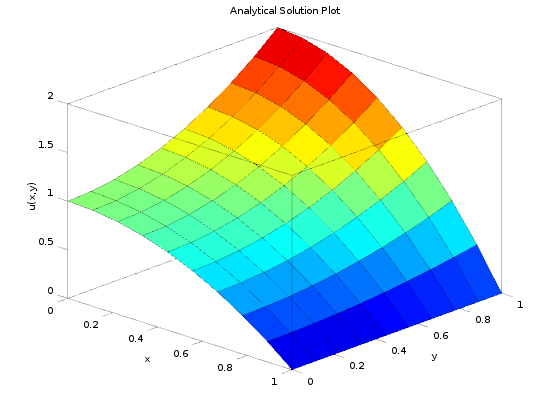
\includegraphics{pois_ana}}
    \subfigure[Steepest Decent Solution]{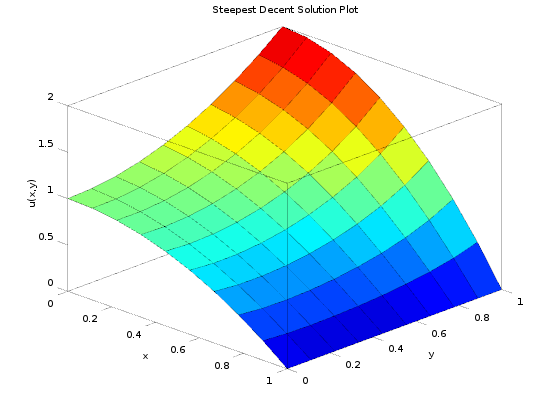
\includegraphics{pois_sd}}
    \subfigure[Liebmann Solution]{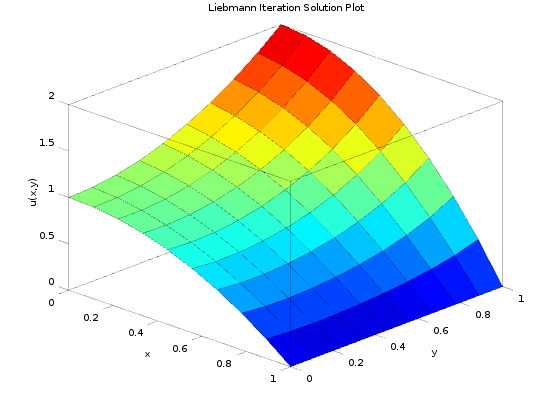
\includegraphics{pois_lieb}}
  \end{subfigmatrix}
 \label{f:p_results}
\end{figure}

\begin{figure}[htb]% order of placement preference: here, top, bottom
  \caption{Convergence plot from the solution of the 10x10 grid}
  \begin{subfigmatrix}{2}
    \subfigure[Steepest Decent error vs iteration]{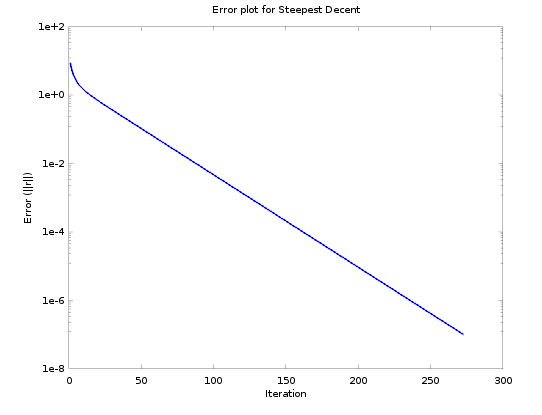
\includegraphics{sd_err}}
    \subfigure[Liebmann error vs iteration]{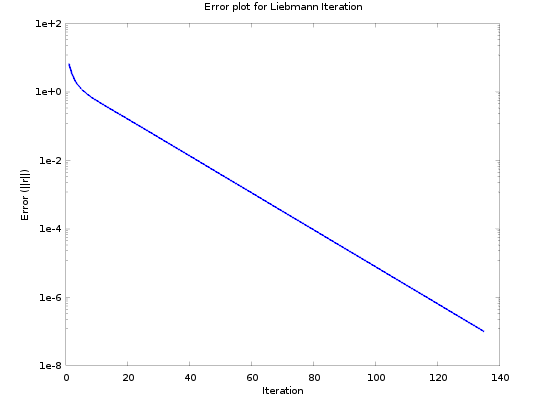
\includegraphics{lieb_err}}
  \end{subfigmatrix}
 \label{f:p_convergeplot}
\end{figure}

\FloatBarrier\subsection{Error-Time-Iterations}
The error of the solutions produced was compared using the average of all the calculated nodes from both the analytical solution and the numerical solution. The figure~\ref{f:err_plot}

\begin{figure}[htb]% order of placement preference: here, top, bottom
  \caption{Convergence plot from the solution of the 10x10 grid}
  \begin{subfigmatrix}{2}
    \subfigure[Iteration vs N]{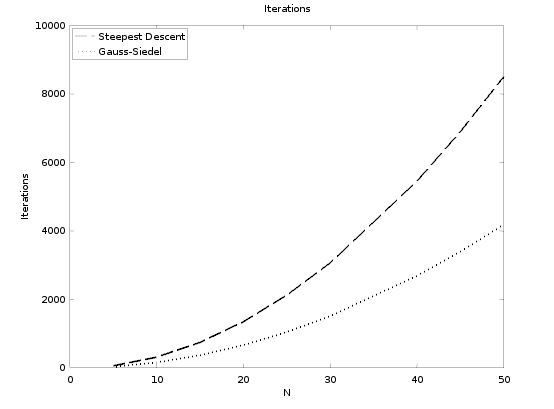
\includegraphics{iterations_study}}
    \subfigure[Time vs N]{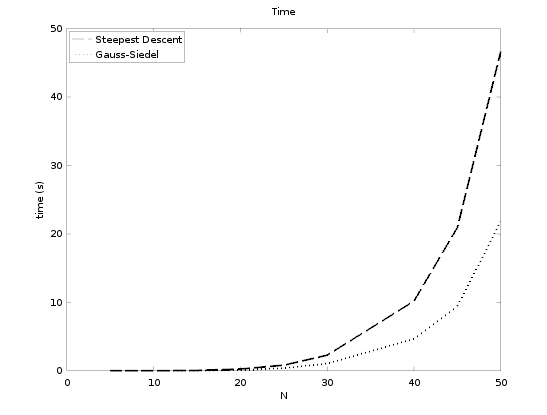
\includegraphics{time_study}}
    \subfigure[Total Error vs N]{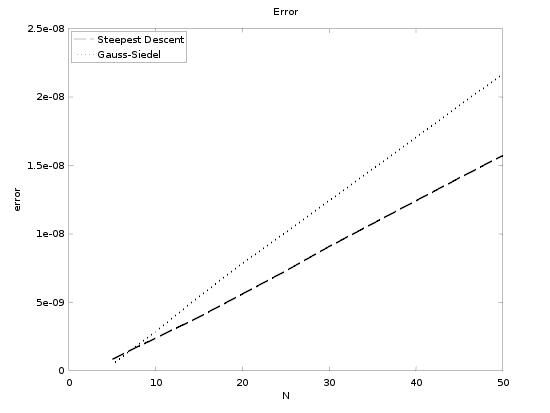
\includegraphics{err_study}}
  \end{subfigmatrix}
 \label{f:p_convergeplot}
\end{figure}

\FloatBarrier\section{Conclusion}
In conclusion we found that our implementation of the Gauss-Siedel out performs the Steepest Decent method. At this point, the data structures and solvers have been optimized to the highest reasonable level without considering full code rewrites. It utilizes pointer to element access and and we realized that pointer access was better than the base accessors and mutators.


\begin{thebibliography}{9}% maximum number of references (for label width)
 \bibitem{holmes:07bk}
 Holmes, M. H., {\it Introduction to numerical mehtods in differential equations}, New York, London: Springer, 2007.

\bibitem{chapraetal:15bk}
Chapra, S. C., and Canale, R. P., {\it Numerical Methods for Engineers}, McGraw-Hill, 2015.

\bibitem{cfdonline:web}
“Numerical methods,” {\it -- CFD-Wiki, the free CFD reference} Available: \verb+http://www.cfd-online.com/wiki/numerical_methods+.

\bibitem{bartnack:94bk}
Barton, J. J., and Nackman, L. R., {\it Scientific and engineering C⁺: an introduction with advanced techniques and examples}, Reading, MA: Addison-Wesley, 1994.

\end{thebibliography}

\section*{Appendix}

\lstinputlisting[caption=g++ with O3 optimization flag]{../outputgpp}
\lstinputlisting[caption=g++ with Ofast optimization flag]{../outputgppfast}
\lstinputlisting[caption=clang++ with O3 optimization flag]{../outputclang}

\end{document}

% - Release $Name:  $ -
